% ----------------------------------------------------------------- %
%             The Speech Signal Processing Toolkit (SPTK)           %
%             developed by SPTK Working Group                       %
%             http://sp-tk.sourceforge.net/                         %
% ----------------------------------------------------------------- %
%                                                                   %
%  Copyright (c) 1984-2007  Tokyo Institute of Technology           %
%                           Interdisciplinary Graduate School of    %
%                           Science and Engineering                 %
%                                                                   %
%                1996-2011  Nagoya Institute of Technology          %
%                           Department of Computer Science          %
%                                                                   %
% All rights reserved.                                              %
%                                                                   %
% Redistribution and use in source and binary forms, with or        %
% without modification, are permitted provided that the following   %
% conditions are met:                                               %
%                                                                   %
% - Redistributions of source code must retain the above copyright  %
%   notice, this list of conditions and the following disclaimer.   %
% - Redistributions in binary form must reproduce the above         %
%   copyright notice, this list of conditions and the following     %
%   disclaimer in the documentation and/or other materials provided %
%   with the distribution.                                          %
% - Neither the name of the SPTK working group nor the names of its %
%   contributors may be used to endorse or promote products derived %
%   from this software without specific prior written permission.   %
%                                                                   %
% THIS SOFTWARE IS PROVIDED BY THE COPYRIGHT HOLDERS AND            %
% CONTRIBUTORS "AS IS" AND ANY EXPRESS OR IMPLIED WARRANTIES,       %
% INCLUDING, BUT NOT LIMITED TO, THE IMPLIED WARRANTIES OF          %
% MERCHANTABILITY AND FITNESS FOR A PARTICULAR PURPOSE ARE          %
% DISCLAIMED. IN NO EVENT SHALL THE COPYRIGHT OWNER OR CONTRIBUTORS %
% BE LIABLE FOR ANY DIRECT, INDIRECT, INCIDENTAL, SPECIAL,          %
% EXEMPLARY, OR CONSEQUENTIAL DAMAGES (INCLUDING, BUT NOT LIMITED   %
% TO, PROCUREMENT OF SUBSTITUTE GOODS OR SERVICES; LOSS OF USE,     %
% DATA, OR PROFITS; OR BUSINESS INTERRUPTION) HOWEVER CAUSED AND ON %
% ANY THEORY OF LIABILITY, WHETHER IN CONTRACT, STRICT LIABILITY,   %
% OR TORT (INCLUDING NEGLIGENCE OR OTHERWISE) ARISING IN ANY WAY    %
% OUT OF THE USE OF THIS SOFTWARE, EVEN IF ADVISED OF THE           %
% POSSIBILITY OF SUCH DAMAGE.                                       %
% ----------------------------------------------------------------- %
\hypertarget{merge}{}
\name{merge}{data merge}{data operation}

\begin{synopsis}
 \item[merge] [ --s $S$ ] [ --l $L_1$ ] [ --n $N_1$ ] [ --L $L_2$ ]
 [ --N $N_2$ ]
 \item[\ ~~~]  [ --o ] [ +{\em type} ] {\em file1} [ {\em infile} ] 
\end{synopsis}

\begin{qsection}{DESCRIPTION}
{\em merge} merges, on a frame-by-frame basis, data from {\em file1} 
into the data from {\em infile} (or standard input), 
sending the result to standard output, as described below.

\hspace{1cm}\includegraphics{fig/merge.eps}
\end{qsection}

\begin{options}
	\argm{s}{S}{insert point}{0}
	\argm{l}{L_1}{frame length of input data}{25}
	\argm{n}{N_1}{order of input data}{$L_1-1$}
	\argm{L}{L_2}{frame length of insert data}{10}
	\argm{N}{N_2}{order of insert data}{$L_2-1$}
	\argm{o}{}{overwrite mode}{FALSE}
	\argp{t}{input data format\\ 
		\begin{tabular}{llcll} \\[-1ex]
         c & char (1 byte) & \quad &
         C & unsigned char (1 byte) \\
         s & short (2 bytes) & \quad &
                     S & unsigned short (2 bytes) \\
         i3 & int (3 bytes) & \quad &
                     I3 & unsigned int (3 bytes) \\
         i & int (4 bytes) & \quad &
                     I & unsigned int (4 bytes) \\
         l & long (4 bytes) & \quad &
                     L & unsigned long (4 bytes) \\
         le & long long (8 bytes) & \quad &
                     LE & unsigned long long (8 bytes) \\
         f & float (4 bytes) & \quad &
                     d & double (8 bytes) \\
		\end{tabular}\\\hspace*{\fill}}{f}
\end{options}


\begin{qsection}{EXAMPLE}
The following example inserts blocks of 2 samples from {\em data.f2}
in short format into {\em data.f1}, also in short format,
the frame length of the file {\em data.f1} is 3, and the blocks
from {\em data.f2} will be inserted from the 3rd sample of
every frame.
The result is {\em data.merge}.
\begin{quote}
 \verb!merge +f -s 2 -l 3 -L 2 +s data.f2 < data.f1 > data.merge!
\end{quote}
For example, if the {\em data.f1} file is 
\[ 1,1,1,2,2,2,\dots \], 
and the {\em data.f2} file is 
\[ 2,3,5,6,\dots \]
then the output {\em data.merge} will be 
\[ 1,1,2,3,1,~ 2,2,5,6,2,\dots \] 

The next example overwrites blocks of 2 samples from {\em data.f2}
in long format into {\em data.f1}, also in long format,
the frame length of the file {\em data.f1} is 4, and the blocks
from {\em data.f2} will be inserted from the 2nd sample of
every frame.
The result is {\em data.merge}.
\begin{quote}
 \verb!merge +f -s 2 -l 4 -L 2 +l -o data.f2 < data.f1 > data.merge!
\end{quote}
For example, if the {\em data.f1} file is 
\[ 1,1,1,1,2,2,2,2,\dots \], 
and the {\em data.f2} file is 
\[ 3,4,5,6,\dots \]
then the output {\em data.merge} will be 
\[  1,3,4,1,~ 2,5,6,2,\dots \] 

\end{qsection}

\begin{qsection}{SEE ALSO}
\hyperlink{bcp}{bcp}
\end{qsection}
